\documentclass[11pt]{article}
\usepackage{ACL}
\usepackage{times}
\usepackage{url}
\usepackage{latexsym}
\usepackage{enumitem}
\usepackage{subfigure}
\usepackage{graphicx}
%%%%% NEW MATH DEFINITIONS %%%%%

\usepackage{amsmath,amsfonts,bm}

% Mark sections of captions for referring to divisions of figures
\newcommand{\figleft}{{\em (Left)}}
\newcommand{\figcenter}{{\em (Center)}}
\newcommand{\figright}{{\em (Right)}}
\newcommand{\figtop}{{\em (Top)}}
\newcommand{\figbottom}{{\em (Bottom)}}
\newcommand{\captiona}{{\em (a)}}
\newcommand{\captionb}{{\em (b)}}
\newcommand{\captionc}{{\em (c)}}
\newcommand{\captiond}{{\em (d)}}

% Highlight a newly defined term
\newcommand{\newterm}[1]{{\bf #1}}


% Figure reference, lower-case.
\def\figref#1{figure~\ref{#1}}
% Figure reference, capital. For start of sentence
\def\Figref#1{Figure~\ref{#1}}
\def\twofigref#1#2{figures \ref{#1} and \ref{#2}}
\def\quadfigref#1#2#3#4{figures \ref{#1}, \ref{#2}, \ref{#3} and \ref{#4}}
% Section reference, lower-case.
\def\secref#1{section~\ref{#1}}
% Section reference, capital.
\def\Secref#1{Section~\ref{#1}}
% Reference to two sections.
\def\twosecrefs#1#2{sections \ref{#1} and \ref{#2}}
% Reference to three sections.
\def\secrefs#1#2#3{sections \ref{#1}, \ref{#2} and \ref{#3}}
% Reference to an equation, lower-case.
\def\eqref#1{equation~\ref{#1}}
% Reference to an equation, upper case
\def\Eqref#1{Equation~\ref{#1}}
% A raw reference to an equation---avoid using if possible
\def\plaineqref#1{\ref{#1}}
% Reference to a chapter, lower-case.
\def\chapref#1{chapter~\ref{#1}}
% Reference to an equation, upper case.
\def\Chapref#1{Chapter~\ref{#1}}
% Reference to a range of chapters
\def\rangechapref#1#2{chapters\ref{#1}--\ref{#2}}
% Reference to an algorithm, lower-case.
\def\algref#1{algorithm~\ref{#1}}
% Reference to an algorithm, upper case.
\def\Algref#1{Algorithm~\ref{#1}}
\def\twoalgref#1#2{algorithms \ref{#1} and \ref{#2}}
\def\Twoalgref#1#2{Algorithms \ref{#1} and \ref{#2}}
% Reference to a part, lower case
\def\partref#1{part~\ref{#1}}
% Reference to a part, upper case
\def\Partref#1{Part~\ref{#1}}
\def\twopartref#1#2{parts \ref{#1} and \ref{#2}}

\def\ceil#1{\lceil #1 \rceil}
\def\floor#1{\lfloor #1 \rfloor}
\def\1{\bm{1}}
\newcommand{\train}{\mathcal{D}}
\newcommand{\valid}{\mathcal{D_{\mathrm{valid}}}}
\newcommand{\test}{\mathcal{D_{\mathrm{test}}}}

\def\eps{{\epsilon}}


% Random variables
\def\reta{{\textnormal{$\eta$}}}
\def\ra{{\textnormal{a}}}
\def\rb{{\textnormal{b}}}
\def\rc{{\textnormal{c}}}
\def\rd{{\textnormal{d}}}
\def\re{{\textnormal{e}}}
\def\rf{{\textnormal{f}}}
\def\rg{{\textnormal{g}}}
\def\rh{{\textnormal{h}}}
\def\ri{{\textnormal{i}}}
\def\rj{{\textnormal{j}}}
\def\rk{{\textnormal{k}}}
\def\rl{{\textnormal{l}}}
% rm is already a command, just don't name any random variables m
\def\rn{{\textnormal{n}}}
\def\ro{{\textnormal{o}}}
\def\rp{{\textnormal{p}}}
\def\rq{{\textnormal{q}}}
\def\rr{{\textnormal{r}}}
\def\rs{{\textnormal{s}}}
\def\rt{{\textnormal{t}}}
\def\ru{{\textnormal{u}}}
\def\rv{{\textnormal{v}}}
\def\rw{{\textnormal{w}}}
\def\rx{{\textnormal{x}}}
\def\ry{{\textnormal{y}}}
\def\rz{{\textnormal{z}}}

% Random vectors
\def\rvepsilon{{\mathbf{\epsilon}}}
\def\rvtheta{{\mathbf{\theta}}}
\def\rva{{\mathbf{a}}}
\def\rvb{{\mathbf{b}}}
\def\rvc{{\mathbf{c}}}
\def\rvd{{\mathbf{d}}}
\def\rve{{\mathbf{e}}}
\def\rvf{{\mathbf{f}}}
\def\rvg{{\mathbf{g}}}
\def\rvh{{\mathbf{h}}}
\def\rvu{{\mathbf{i}}}
\def\rvj{{\mathbf{j}}}
\def\rvk{{\mathbf{k}}}
\def\rvl{{\mathbf{l}}}
\def\rvm{{\mathbf{m}}}
\def\rvn{{\mathbf{n}}}
\def\rvo{{\mathbf{o}}}
\def\rvp{{\mathbf{p}}}
\def\rvq{{\mathbf{q}}}
\def\rvr{{\mathbf{r}}}
\def\rvs{{\mathbf{s}}}
\def\rvt{{\mathbf{t}}}
\def\rvu{{\mathbf{u}}}
\def\rvv{{\mathbf{v}}}
\def\rvw{{\mathbf{w}}}
\def\rvx{{\mathbf{x}}}
\def\rvy{{\mathbf{y}}}
\def\rvz{{\mathbf{z}}}

% Elements of random vectors
\def\erva{{\textnormal{a}}}
\def\ervb{{\textnormal{b}}}
\def\ervc{{\textnormal{c}}}
\def\ervd{{\textnormal{d}}}
\def\erve{{\textnormal{e}}}
\def\ervf{{\textnormal{f}}}
\def\ervg{{\textnormal{g}}}
\def\ervh{{\textnormal{h}}}
\def\ervi{{\textnormal{i}}}
\def\ervj{{\textnormal{j}}}
\def\ervk{{\textnormal{k}}}
\def\ervl{{\textnormal{l}}}
\def\ervm{{\textnormal{m}}}
\def\ervn{{\textnormal{n}}}
\def\ervo{{\textnormal{o}}}
\def\ervp{{\textnormal{p}}}
\def\ervq{{\textnormal{q}}}
\def\ervr{{\textnormal{r}}}
\def\ervs{{\textnormal{s}}}
\def\ervt{{\textnormal{t}}}
\def\ervu{{\textnormal{u}}}
\def\ervv{{\textnormal{v}}}
\def\ervw{{\textnormal{w}}}
\def\ervx{{\textnormal{x}}}
\def\ervy{{\textnormal{y}}}
\def\ervz{{\textnormal{z}}}

% Random matrices
\def\rmA{{\mathbf{A}}}
\def\rmB{{\mathbf{B}}}
\def\rmC{{\mathbf{C}}}
\def\rmD{{\mathbf{D}}}
\def\rmE{{\mathbf{E}}}
\def\rmF{{\mathbf{F}}}
\def\rmG{{\mathbf{G}}}
\def\rmH{{\mathbf{H}}}
\def\rmI{{\mathbf{I}}}
\def\rmJ{{\mathbf{J}}}
\def\rmK{{\mathbf{K}}}
\def\rmL{{\mathbf{L}}}
\def\rmM{{\mathbf{M}}}
\def\rmN{{\mathbf{N}}}
\def\rmO{{\mathbf{O}}}
\def\rmP{{\mathbf{P}}}
\def\rmQ{{\mathbf{Q}}}
\def\rmR{{\mathbf{R}}}
\def\rmS{{\mathbf{S}}}
\def\rmT{{\mathbf{T}}}
\def\rmU{{\mathbf{U}}}
\def\rmV{{\mathbf{V}}}
\def\rmW{{\mathbf{W}}}
\def\rmX{{\mathbf{X}}}
\def\rmY{{\mathbf{Y}}}
\def\rmZ{{\mathbf{Z}}}

% Elements of random matrices
\def\ermA{{\textnormal{A}}}
\def\ermB{{\textnormal{B}}}
\def\ermC{{\textnormal{C}}}
\def\ermD{{\textnormal{D}}}
\def\ermE{{\textnormal{E}}}
\def\ermF{{\textnormal{F}}}
\def\ermG{{\textnormal{G}}}
\def\ermH{{\textnormal{H}}}
\def\ermI{{\textnormal{I}}}
\def\ermJ{{\textnormal{J}}}
\def\ermK{{\textnormal{K}}}
\def\ermL{{\textnormal{L}}}
\def\ermM{{\textnormal{M}}}
\def\ermN{{\textnormal{N}}}
\def\ermO{{\textnormal{O}}}
\def\ermP{{\textnormal{P}}}
\def\ermQ{{\textnormal{Q}}}
\def\ermR{{\textnormal{R}}}
\def\ermS{{\textnormal{S}}}
\def\ermT{{\textnormal{T}}}
\def\ermU{{\textnormal{U}}}
\def\ermV{{\textnormal{V}}}
\def\ermW{{\textnormal{W}}}
\def\ermX{{\textnormal{X}}}
\def\ermY{{\textnormal{Y}}}
\def\ermZ{{\textnormal{Z}}}

% Vectors
\def\vzero{{\bm{0}}}
\def\vone{{\bm{1}}}
\def\vmu{{\bm{\mu}}}
\def\vtheta{{\bm{\theta}}}
\def\va{{\bm{a}}}
\def\vb{{\bm{b}}}
\def\vc{{\bm{c}}}
\def\vd{{\bm{d}}}
\def\ve{{\bm{e}}}
\def\vf{{\bm{f}}}
\def\vg{{\bm{g}}}
\def\vh{{\bm{h}}}
\def\vi{{\bm{i}}}
\def\vj{{\bm{j}}}
\def\vk{{\bm{k}}}
\def\vl{{\bm{l}}}
\def\vm{{\bm{m}}}
\def\vn{{\bm{n}}}
\def\vo{{\bm{o}}}
\def\vp{{\bm{p}}}
\def\vq{{\bm{q}}}
\def\vr{{\bm{r}}}
\def\vs{{\bm{s}}}
\def\vt{{\bm{t}}}
\def\vu{{\bm{u}}}
\def\vv{{\bm{v}}}
\def\vw{{\bm{w}}}
\def\vx{{\bm{x}}}
\def\vy{{\bm{y}}}
\def\vz{{\bm{z}}}

% Elements of vectors
\def\evalpha{{\alpha}}
\def\evbeta{{\beta}}
\def\evepsilon{{\epsilon}}
\def\evlambda{{\lambda}}
\def\evomega{{\omega}}
\def\evmu{{\mu}}
\def\evpsi{{\psi}}
\def\evsigma{{\sigma}}
\def\evtheta{{\theta}}
\def\eva{{a}}
\def\evb{{b}}
\def\evc{{c}}
\def\evd{{d}}
\def\eve{{e}}
\def\evf{{f}}
\def\evg{{g}}
\def\evh{{h}}
\def\evi{{i}}
\def\evj{{j}}
\def\evk{{k}}
\def\evl{{l}}
\def\evm{{m}}
\def\evn{{n}}
\def\evo{{o}}
\def\evp{{p}}
\def\evq{{q}}
\def\evr{{r}}
\def\evs{{s}}
\def\evt{{t}}
\def\evu{{u}}
\def\evv{{v}}
\def\evw{{w}}
\def\evx{{x}}
\def\evy{{y}}
\def\evz{{z}}

% Matrix
\def\mA{{\bm{A}}}
\def\mB{{\bm{B}}}
\def\mC{{\bm{C}}}
\def\mD{{\bm{D}}}
\def\mE{{\bm{E}}}
\def\mF{{\bm{F}}}
\def\mG{{\bm{G}}}
\def\mH{{\bm{H}}}
\def\mI{{\bm{I}}}
\def\mJ{{\bm{J}}}
\def\mK{{\bm{K}}}
\def\mL{{\bm{L}}}
\def\mM{{\bm{M}}}
\def\mN{{\bm{N}}}
\def\mO{{\bm{O}}}
\def\mP{{\bm{P}}}
\def\mQ{{\bm{Q}}}
\def\mR{{\bm{R}}}
\def\mS{{\bm{S}}}
\def\mT{{\bm{T}}}
\def\mU{{\bm{U}}}
\def\mV{{\bm{V}}}
\def\mW{{\bm{W}}}
\def\mX{{\bm{X}}}
\def\mY{{\bm{Y}}}
\def\mZ{{\bm{Z}}}
\def\mBeta{{\bm{\beta}}}
\def\mPhi{{\bm{\Phi}}}
\def\mLambda{{\bm{\Lambda}}}
\def\mSigma{{\bm{\Sigma}}}

% Tensor
\DeclareMathAlphabet{\mathsfit}{\encodingdefault}{\sfdefault}{m}{sl}
\SetMathAlphabet{\mathsfit}{bold}{\encodingdefault}{\sfdefault}{bx}{n}
\newcommand{\tens}[1]{\bm{\mathsfit{#1}}}
\def\tA{{\tens{A}}}
\def\tB{{\tens{B}}}
\def\tC{{\tens{C}}}
\def\tD{{\tens{D}}}
\def\tE{{\tens{E}}}
\def\tF{{\tens{F}}}
\def\tG{{\tens{G}}}
\def\tH{{\tens{H}}}
\def\tI{{\tens{I}}}
\def\tJ{{\tens{J}}}
\def\tK{{\tens{K}}}
\def\tL{{\tens{L}}}
\def\tM{{\tens{M}}}
\def\tN{{\tens{N}}}
\def\tO{{\tens{O}}}
\def\tP{{\tens{P}}}
\def\tQ{{\tens{Q}}}
\def\tR{{\tens{R}}}
\def\tS{{\tens{S}}}
\def\tT{{\tens{T}}}
\def\tU{{\tens{U}}}
\def\tV{{\tens{V}}}
\def\tW{{\tens{W}}}
\def\tX{{\tens{X}}}
\def\tY{{\tens{Y}}}
\def\tZ{{\tens{Z}}}


% Graph
\def\gA{{\mathcal{A}}}
\def\gB{{\mathcal{B}}}
\def\gC{{\mathcal{C}}}
\def\gD{{\mathcal{D}}}
\def\gE{{\mathcal{E}}}
\def\gF{{\mathcal{F}}}
\def\gG{{\mathcal{G}}}
\def\gH{{\mathcal{H}}}
\def\gI{{\mathcal{I}}}
\def\gJ{{\mathcal{J}}}
\def\gK{{\mathcal{K}}}
\def\gL{{\mathcal{L}}}
\def\gM{{\mathcal{M}}}
\def\gN{{\mathcal{N}}}
\def\gO{{\mathcal{O}}}
\def\gP{{\mathcal{P}}}
\def\gQ{{\mathcal{Q}}}
\def\gR{{\mathcal{R}}}
\def\gS{{\mathcal{S}}}
\def\gT{{\mathcal{T}}}
\def\gU{{\mathcal{U}}}
\def\gV{{\mathcal{V}}}
\def\gW{{\mathcal{W}}}
\def\gX{{\mathcal{X}}}
\def\gY{{\mathcal{Y}}}
\def\gZ{{\mathcal{Z}}}

% Sets
\def\sA{{\mathbb{A}}}
\def\sB{{\mathbb{B}}}
\def\sC{{\mathbb{C}}}
\def\sD{{\mathbb{D}}}
% Don't use a set called E, because this would be the same as our symbol
% for expectation.
\def\sF{{\mathbb{F}}}
\def\sG{{\mathbb{G}}}
\def\sH{{\mathbb{H}}}
\def\sI{{\mathbb{I}}}
\def\sJ{{\mathbb{J}}}
\def\sK{{\mathbb{K}}}
\def\sL{{\mathbb{L}}}
\def\sM{{\mathbb{M}}}
\def\sN{{\mathbb{N}}}
\def\sO{{\mathbb{O}}}
\def\sP{{\mathbb{P}}}
\def\sQ{{\mathbb{Q}}}
\def\sR{{\mathbb{R}}}
\def\sS{{\mathbb{S}}}
\def\sT{{\mathbb{T}}}
\def\sU{{\mathbb{U}}}
\def\sV{{\mathbb{V}}}
\def\sW{{\mathbb{W}}}
\def\sX{{\mathbb{X}}}
\def\sY{{\mathbb{Y}}}
\def\sZ{{\mathbb{Z}}}

% Entries of a matrix
\def\emLambda{{\Lambda}}
\def\emA{{A}}
\def\emB{{B}}
\def\emC{{C}}
\def\emD{{D}}
\def\emE{{E}}
\def\emF{{F}}
\def\emG{{G}}
\def\emH{{H}}
\def\emI{{I}}
\def\emJ{{J}}
\def\emK{{K}}
\def\emL{{L}}
\def\emM{{M}}
\def\emN{{N}}
\def\emO{{O}}
\def\emP{{P}}
\def\emQ{{Q}}
\def\emR{{R}}
\def\emS{{S}}
\def\emT{{T}}
\def\emU{{U}}
\def\emV{{V}}
\def\emW{{W}}
\def\emX{{X}}
\def\emY{{Y}}
\def\emZ{{Z}}
\def\emSigma{{\Sigma}}

% entries of a tensor
% Same font as tensor, without \bm wrapper
\newcommand{\etens}[1]{\mathsfit{#1}}
\def\etLambda{{\etens{\Lambda}}}
\def\etA{{\etens{A}}}
\def\etB{{\etens{B}}}
\def\etC{{\etens{C}}}
\def\etD{{\etens{D}}}
\def\etE{{\etens{E}}}
\def\etF{{\etens{F}}}
\def\etG{{\etens{G}}}
\def\etH{{\etens{H}}}
\def\etI{{\etens{I}}}
\def\etJ{{\etens{J}}}
\def\etK{{\etens{K}}}
\def\etL{{\etens{L}}}
\def\etM{{\etens{M}}}
\def\etN{{\etens{N}}}
\def\etO{{\etens{O}}}
\def\etP{{\etens{P}}}
\def\etQ{{\etens{Q}}}
\def\etR{{\etens{R}}}
\def\etS{{\etens{S}}}
\def\etT{{\etens{T}}}
\def\etU{{\etens{U}}}
\def\etV{{\etens{V}}}
\def\etW{{\etens{W}}}
\def\etX{{\etens{X}}}
\def\etY{{\etens{Y}}}
\def\etZ{{\etens{Z}}}

% The true underlying data generating distribution
\newcommand{\pdata}{p_{\rm{data}}}
% The empirical distribution defined by the training set
\newcommand{\ptrain}{\hat{p}_{\rm{data}}}
\newcommand{\Ptrain}{\hat{P}_{\rm{data}}}
% The model distribution
\newcommand{\pmodel}{p_{\rm{model}}}
\newcommand{\Pmodel}{P_{\rm{model}}}
\newcommand{\ptildemodel}{\tilde{p}_{\rm{model}}}
% Stochastic autoencoder distributions
\newcommand{\pencode}{p_{\rm{encoder}}}
\newcommand{\pdecode}{p_{\rm{decoder}}}
\newcommand{\precons}{p_{\rm{reconstruct}}}

\newcommand{\laplace}{\mathrm{Laplace}} % Laplace distribution

\DeclareMathOperator{\E}{\mathbb{E}}
\newcommand{\Ls}{\mathcal{L}}
\newcommand{\R}{\mathbb{R}}
\newcommand{\emp}{\tilde{p}}
\newcommand{\lr}{\alpha}
\newcommand{\reg}{\lambda}
\newcommand{\rect}{\mathrm{rectifier}}
\newcommand{\softmax}{\mathrm{softmax}}
\newcommand{\sigmoid}{\sigma}
\newcommand{\softplus}{\zeta}
\newcommand{\KL}{D_{\mathrm{KL}}}
\newcommand{\Var}{\mathrm{Var}}
\newcommand{\standarderror}{\mathrm{SE}}
\newcommand{\Cov}{\mathrm{Cov}}
% Wolfram Mathworld says $L^2$ is for function spaces and $\ell^2$ is for vectors
% But then they seem to use $L^2$ for vectors throughout the site, and so does
% wikipedia.
\newcommand{\normlzero}{L^0}
\newcommand{\normlone}{L^1}
\newcommand{\normltwo}{L^2}
\newcommand{\normlp}{L^p}
\newcommand{\normmax}{L^\infty}

\newcommand{\parents}{Pa} % See usage in notation.tex. Chosen to match Daphne's book.

\DeclareMathOperator*{\argmax}{arg\,max}
\DeclareMathOperator*{\argmin}{arg\,min}

\DeclareMathOperator{\sign}{sign}
\DeclareMathOperator{\Tr}{Tr}
\let\ab\allowbreak

\usepackage{bbm}
\usepackage{amssymb}
\usepackage{amsmath}
\allowdisplaybreaks
\usepackage{cancel}
\usepackage[switch]{lineno}
\usepackage[bottom]{footmisc}
\usepackage[ruled,vlined]{algorithm2e}

\definecolor{orange}{rgb}{0.93, 0.53, 0.18}

\aclfinalcopy % Uncomment this line for the final submission
%\def\aclpaperid{***} %  Enter the acl Paper ID here


\title{Modelling Language Communication and Learning with \\ Rate Distortion Theory}

\author{Team members} 

% 2. Two rows of authors (set titlebox length to 7cm)
%
% \author{First Author \\
%  Affiliation / Address line 1 \\
%  Affiliation / Address line 2 \\
%  Affiliation / Address line 3 \\
%  {\tt email@domain} \\\And
%  Second Author \\
%  Affiliation / Address line 1 \\
%  Affiliation / Address line 2 \\
%  Affiliation / Address line 3 \\
%  {\tt email@domain} \\\AND
%  Third Author \\
%  Affiliation / Address line 1 \\
%  Affiliation / Address line 2 \\
%  Affiliation / Address line 3 \\
%  {\tt email@domain} \\\And
%  Fourth Author \\
%  Affiliation / Address line 1 \\
%  Affiliation / Address line 2 \\
%  Affiliation / Address line 3 \\
%  {\tt email@domain} \\}
%
% 3. More than four authors (set titlebox length to 7cm or more)
%
%\author{First Author$^{1}$, Second Author$^{2}$, Third Author$^{3}$, Fourth Author$^{1,4}$,\\
%\textbf{Fifth Author$^{2}$, Sixth Author$^{5}$, Seventh Author$^{6}$, Eighth Author$^{7}$}\\
%[0.5cm] 
%$^{1}$Affiliation 1, Affiliation / Address line 2, Affiliation / Address line 3, {\tt email@domain} \\
%$^{2}$Affiliation 2, Affiliation / Address line 2, Affiliation / Address line 3, {\tt email@domain} \\
%$^{3}$Affiliation 3, Affiliation / Address line 2, Affiliation / Address line 3, {\tt email@domain} \\
%$^{4}$Affiliation 4, Affiliation / Address line 2, Affiliation / Address line 3, {\tt email@domain} \\
%$^{5}$Affiliation 5, Affiliation / Address line 2, Affiliation / Address line 3, {\tt email@domain} \\
%$^{6}$Affiliation 6, Affiliation / Address line 2, Affiliation / Address line 3, {\tt email@domain} \\
%$^{7}$Affiliation 7, Affiliation / Address line 2, Affiliation / Address line 3, {\tt email@domain} \\}
%
\date{}

\begin{document}
\maketitle
\linenumbers
\begin{abstract}
  This document describes the basic concepts and [to be written].
\end{abstract}

\section{Universal Components}
\label{sec:uni_components}

% \subsection{Variables and Functions}
% \label{ssec:vars_funcs}

The variables involved in this project are listed as follows:

\begin{itemize}[leftmargin=*]
    \item \textbf{meaning $M$\footnote{In this document, a random variable is notated by a capital letter, e.g. $M$ here, its possible values are notated by the corresponding lower case letter, e.g. $m$, and the set of its sample space is notated by the corresponding calligraphic capital letter, e.g. $\mathcal{M}$.}}: a meaning $m\in\mathcal{M}$ is \textcolor{red}{a discrete variable} indicating the possible meanings.
    It specifies both distributions over $c$, i.e. $p(c|m)$, and distributions over words $w$, i.e. $p(w|m)$.
    In fact, \textcolor{red}{$M$ is the core variable in our project}, and it corresponds to the source variable $X$ in the standard information theory model, \citep[e.g.][]{RDT}.
    
    We don't know the size of meaning space $|\mathcal{M}|$ nor $p(m)$ for each $m$.
    In both communication problem and learning problem, we have to infer that out.
    Or, in the language of probabilistic graphical model, $m$ is a latent variable in our setup.
    We will also show in the Section~\ref{sec:comm}and~\ref{sec:learning} that $p(m)$ can be inferred out by algorithms similar to Expectation-Maximisation. 

    \item \textbf{colour chip $C$}: a colour chip $c\in\mathcal{C}$ is also a discrete integer variable indicating the possible values of colours. 
    $\mathcal{C}$ is given in the data set, and it keeps identical across different languages (defined below). 
    The colour palette $\mathcal{C}$ we're going to use is shown in Figure~\ref{fig:colour_palette}, where each grid corresponds to a specific $c$.
        \begin{figure}[h]
            \centering
            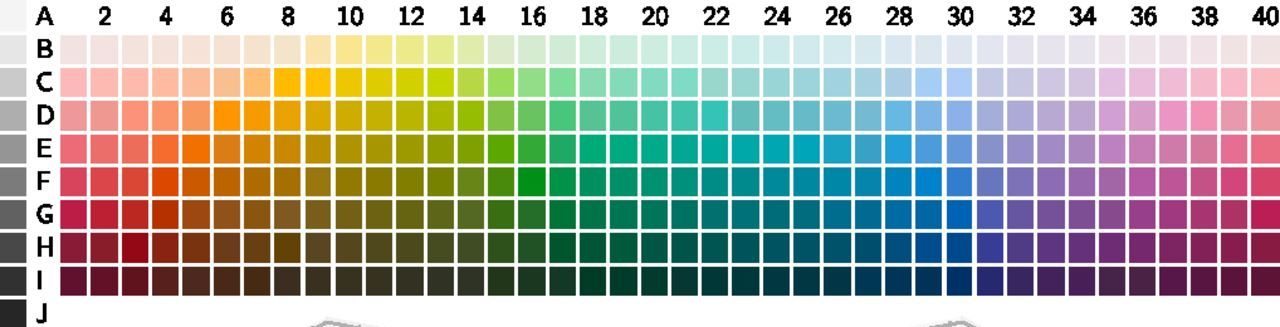
\includegraphics[width=0.49\textwidth]{docs/intro_rate_distortion/graphs/colour_palette.jpg}
            \caption{Colour palette introduced by \citet{berlin1991basic}}
            \label{fig:colour_palette}
        \end{figure}
        
    In this project, we will ignore the variable $u$ (``universe'') used by \citet{zaslavsky2018efficient} because the entire universe is constrained to the colour palette. 
    Mathematically, $\mathcal{U}$ is just a superset of $\mathcal{C}$ which represents the objects in the universe.
    
    Same to \cite{zaslavsky2018efficient}, given a meaning $m$, we assume the conditional distribution of $c$ is a Gaussian centred at $\rc(m)$, i.e.:
    \begin{align}
    p(c|m)\propto \exp{-\frac{1}{\sigma^2}}||c-\rc(m)||^2
    \label{eq:p_c_given_m}
    \end{align}
    
    In practice, we will allocate a ``mode colour chip'' for each meaning $m$, thus we use $\rc(m)$ instead of $m$ in Equation~\ref{eq:p_c_given_m}.
    But, conceptually, it is the same to $\exp{-\frac{1}{\sigma^2}}||c-m||^2$. 
    As you may notice, $m$ has different values from $c$, therefore putting these two together is a bit wired. 
    
    An example is given in Figure~\ref{fig:green_meaning}.
        \begin{figure}[h]
            \centering
            
\includegraphics[width=0.49\textwidth]{docs/intro_rate_distortion/graphs/green_meaning.png}
            \caption{Meaning of ``green'' which is a Gaussian distribution over different colour chips.}
            \label{fig:green_meaning}
        \end{figure}
        
    \item \textbf{word $W$}: a discrete variable transmitted from speaker to listener. 
    We can give each $w\in\mathcal{W}$ a name, e.g. ``blue'' for the 3rd value.
    However, this is not necessary here since we do not care what actual word is used for some meaning. Sometimes, $\mathcal{W}$ is referred to as ``dictionary'', ``vocabulary'', or ``lexicon''.
    Since the conditional distribution $p(w|m)$ has a name and it's an important concept in this project, so we illustrate it in the following separately.
    
    \item \textbf{language $p(w|m)$}: a language is the distribution of words conditioned on meanings, i.e. a language tells us the probability of emitting a word $w$ given a meaning $m$.
    It is a.k.a. the \emph{encoder} in standard information theory terminology, and can also be written as a function $L:\mathcal{M}\rightarrow\mathcal{W}$.
        \begin{figure}[h]
            \centering
            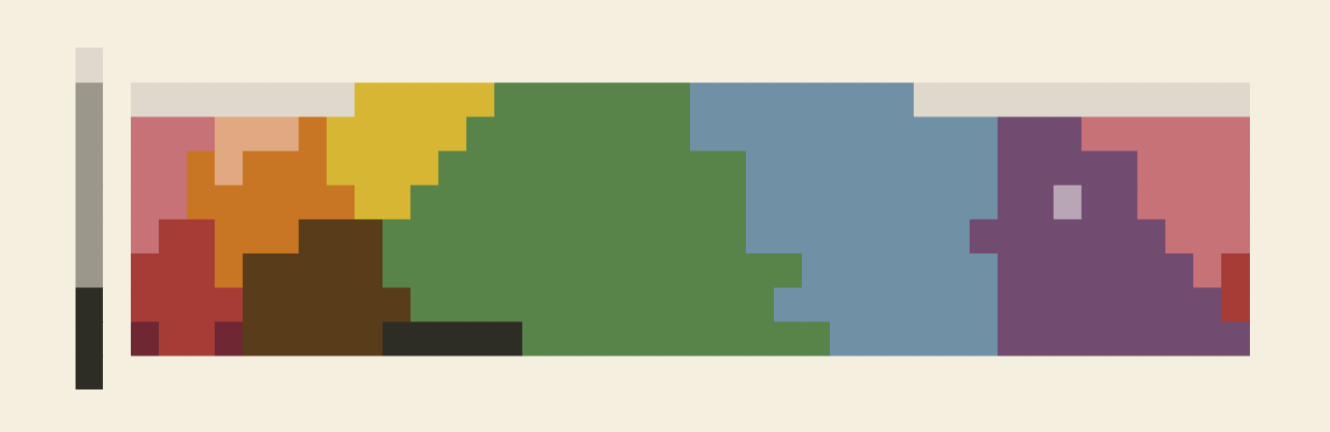
\includegraphics[width=0.49\textwidth]{docs/intro_rate_distortion/graphs/color_language.png}
            \caption{English on the colour palette from \citet{berlin1991basic}.
            }
            \label{fig:language_example}
        \end{figure}
    
    An example based on English is illustrated in Figure~\ref{fig:language_example}.
    To be specific, the colour chips in the green region will all be referred by the word ``green''.
    The boundary is hard in this example, but the naming policy $p(w|m)$ can have soft boundaries, e.g. by using Gaussian distribution.
    
    \item \textbf{interpretation policy $p(\hat{m}|w)$\label{par:decoder}}: an interpretation specifies the distribution of colour chips given a specific word, a.k.a. \emph{decoder} in standard information theory terminology, and can also be written as a function $I:\mathcal{W}\rightarrow\mathcal{C}$.
    Note we use $\hat{m}$ here instead of $m$ because the two random variables have different probability mass although they have the same sample space. 
    $\hat{m}$ is the understood or reconstructed meaning from the word $w$.
    For example, after receiving the word ``green'', we could have a distribution over all colours that is very similar to the one in Figure~\ref{fig:green_meaning} but more skewed towards blue.
    
    Following \citet{zaslavsky2018efficient}, an \textcolor{red}{important assumption} of this project is that mappings between $\hat{m}$ and $w$ are \textcolor{red}{one-to-one}, i.e.
    \begin{equation}
        p(\hat{m}|w) =
        \begin{cases}
            1 & \text{if $\hat{m}=w$}\\
            0 & \text{otherwise}
        \end{cases} 
        \label{eq:bijective_mhat_w}
    \end{equation}
    
    Rigorously speaking, $\hat{m}$ can't equal to $w$, but it is easier to write it this way. Therefore, the equivalence below holds:
    \begin{equation}
        p(c|w)  = \sum_{\hat{m}} p(c|\hat{m})p(\hat{m}|w)  = p(c|\hat{m})
        \label{eq:p_mhat_and_m}
    \end{equation}
    
    Similar to \citep{zaslavsky2018efficient}, by applying Bayes theorem, we can have the following equivalence:
    \begin{equation}
        \begin{split}
            & p(c|\hat{m}) = p(c|w) \\
            & = \sum_m p(c|m)p(m|w) \\
            & = \sum_m p(c|m) \frac{p(w|m)p(m)}{p(w)} \\
            & = \sum_m p(c|m) \frac{p(w|m)p(m)}{\sum_m p(w|m)p(m)}
        \end{split}
        \label{eq:bayesian_interpretation}
    \end{equation}
    That is, we can determine interpretation $p(c|w) = p(c|\hat{m})$ once we have an established language $p(w|m)$ and established meanings probability mass function $p(m)$.
    
    
\end{itemize}

\section{Communication Problem}
\label{sec:comm}

We first illustrate communication problem as there is no unique variable involved in it.
Our aim in the communication part of this project is to produce a diagram similar to the one sketched in Figure~\ref{fig:curve_comm}.
The red line in the figure is referred as ``frontier'', and our aim is to show that it is indeed a trade-off curve.
The calculation of each axes and the curve itself are illustrated in the following subsections.

It is important to note that we are going to \textcolor{red}{optimise both $P(W|M)$ and $P(M)$} in the communication problem to reduce the information loss defined in Section~\ref{ssec:lan_info_loss}.

\begin{figure}[t]
    \centering
    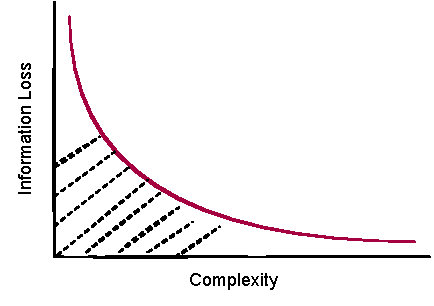
\includegraphics[width=0.49\textwidth]{docs/intro_rate_distortion/graphs/communication_curve.pdf}
    \caption{The curve we aim to plot in the communication problem.}
    \label{fig:curve_comm}
\end{figure}

\subsection{Pipeline in Communication}
\label{ssec:comm_pipeline}

The pipeline of our model is shown in Figure~\ref{fig:pipeline}, where $\mathcal{E}$ denotes the error/loss function we're going to use.
Note that the communication is about transmitting $m$ and reconstructing it as $\hat{m}$, thus there's no $c$ involved in the diagram.
But, to evaluate the information loss during communication, we need $c$ as a part of the metric illustrated in Equation~\ref{eq:comm_loss_function}.

\begin{figure}[h]
    \centering
    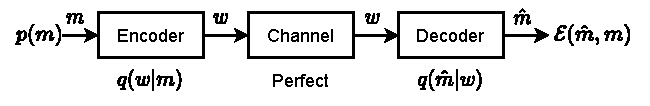
\includegraphics[width=0.49\textwidth]{docs/intro_rate_distortion/graphs/cog_communication.pdf}
    \caption{The pipeline of our model. We follow \citet{zaslavsky2018efficient} to assume that the communication channel is perfect/noise-less.}
    \label{fig:pipeline}
\end{figure}

In the existing works, the common choices of $\mathcal{E}$ are indicator function $\mathbbm{1}(\hat{m}=m)$ and $KL$-divergence $D[p(c|\hat{m})||p(c|m)]$.
since we're going to use $KL$-divergence, the full form of it is given as follow:

\begin{equation}
\begin{split}
    & \mathcal{E}(m,\hat{m}) \triangleq  D[m||\hat{m}] \\
    & = D[p(c|m)||p(c|\hat{m})]  \\
    % & = \sum_{c} q(c|\hat{m}) \log \frac{q(c|\hat{m})}{q(c|m)} \\
    & = \sum_{c} p(c|m) \log \frac{p(c|m)}{p(c|\hat{m})} \\
     & = \sum_{c} p(c|m) \log \frac{p(c|m)}{p(c|\textcolor{red}{w})}
\end{split}
\label{eq:comm_loss_function}
\end{equation}
where the last equivalence holds due to Equation~\ref{eq:p_mhat_and_m}.

The distortion (a.k.a. information loss with $D[m||\hat{m}]$) is then defined by the expectation of our error/loss function, i.e.

\begin{equation}
    \mathbb{E}_{m,\hat{m}}\left[\mathcal{E}(m,\hat{m})\right]
    \label{eq:distortion}
\end{equation}


\subsection{Complexity of Languages}
\label{ssec:complexity}

The complexity of our a language is defined as the mutual information between $m$ and $w$, i.e. 

\begin{equation}
    I(M;W) = \sum_{m,w} p(m)p(w|m)\log \frac{p(w|m)}{p(w)}
    \label{eq:complexity_definition}
\end{equation}

Given $p(m)$, the amount of information conveyed can be measured by its entropy, i.e. $H(M)$.
With $H(M)=I(M;W)+H(M|W)$, it is then straightforward to see that $I(M;W)$ is how many extra information about $m$ conveyed by $w$, i.e. the amount of information conveyed in the channel/language.
Assuming that more information means higher complexity \textcolor{orange}{@Frank: any citation to support this assumption?}, then the complexity of a language can be measured by $I(M;W)$,
or at least, there is a positive correlation between the two quantities.

Therefore, once we have a $p(w|m)$, we can calculate its complexity by simply following Equation~\ref{eq:complexity_definition}.
We will show later how to derive such a $p(w|m)$ in Section~\ref{ssec:comm_opt_ib}.

\subsection{Information Loss of Languages}
\label{ssec:lan_info_loss}

As we illustrated before, given a language and an interpretation policy, we can derive $p(\hat{m}|w)$.
Then, the joint distribution of $\hat{m}$ and $m$ is as follow:

\begin{equation}
    \begin{split}
        p(\hat{m},m) 
        & = p(\hat{m}|m)p(m) \\
        & = \sum_w p(\hat{m}|w)p(w|m)p(m)
    \end{split}
    \label{eq:joint_c_hat_c}
\end{equation}

Combining the above equation with Equation~\ref{eq:distortion}, the information loss can then be calculated as:

\begin{equation}
    \begin{split}
        & \mathbb{E}_{p(\hat{m},m)}\left[D[m||\hat{m}]\right] \\
        & = \mathbb{E}_{p(\hat{m},m)}\left[ \sum_{c} p(c|m) \log \frac{p(c|m)}{p(c|w)} \right] \\
        & = \sum_{\hat{m},m} p(\hat{m},m) \sum_{c} p(c|m) \log \frac{p(c|m)}{p(c|w)} \\
    \end{split}
    \label{eq:comm_info_loss}
\end{equation}

Now, let's further factorise Equation~\ref{eq:comm_info_loss} as follows:

\begin{align*}
    % \begin{aligned}
        & \mathbb{E}_{p(\hat{m},m)}\left[D[m||\hat{m}]\right] \\
        & = \sum_{\hat{m},m,w} p(\hat{m}|w)p(w|m)p(m) \\ 
        & \cdot \sum_{c} p(c|m) \log \frac{p(c|m)}{p(c|w)} \\
        & = \sum_{\hat{m},m,w,c} p(\hat{m}|w)p(w|m)p(m)p(c|m)\log \frac{p(c|m)}{p(c|w)} \\
        & = \sum_{\hat{m},m,w,c} p(\hat{m}|w)p(w|m)p(m)p(c|m) \log p(c|m) \\
        & - \sum_{\hat{m},m,w,c} p(\hat{m}|w)p(w|m)p(m)p(c|m) \log p(c|w) \\ 
        & = \sum_{\hat{m},m,w,c} p(\hat{m}|w)p(w|m)p(m)p(c|m) \log \frac{p(c|m)}{p(c)} \\ 
        & - \sum_{\hat{m},m,w,c} p(\hat{m}|w)p(w|m)p(m)p(c|m) \log \frac{p(c|w)}{p(c)} \\ 
        & = \sum_{\hat{m},m,w,c} p(\hat{m},m,w,c) \log \frac{p(c|m)}{p(c)} \\
        & - \sum_{\hat{m},m,w,c} p(\hat{m},m,w,c) \log \frac{p(c|w)}{p(c)} \\ 
        & = \sum_{\cancel{\hat{m},w},m,c} p(\cancel{\hat{m},w},m,c) \log \frac{p(c|m)}{p(c)} \\ 
        & - \sum_{\cancel{\hat{m},m},w,c} p(\cancel{\hat{m},m},w,c) \log \frac{p(c|w)}{p(c)} \\ 
        & = \sum_{m,c} p(m,c) \log \frac{p(c|m)}{p(c)} \\ 
        & - \sum_{w,c} p(w,c) \log \frac{p(c|w)}{p(c)} \\ 
        & = \textcolor{red}{\sum_{m,c} p(m,c) \log \frac{p(c|m)p(m)}{p(c)p(m)}} \\ 
        & - \textcolor{blue}{\sum_{w,c} p(w,c) \log \frac{p(c|w)p(w)}{p(c)p(w)}} \\  
        & = \textcolor{red}{I(M;C)} - \textcolor{blue}{I(W;C)} 
    % \end{aligned}
    \label{eq:factorise_distortion}
\end{align*}
where the last line corresponds to Equation~[5] in \citep{zaslavsky2018efficient}.

In the above equation, $I(M;C)$ is actually independent of $p(w|m)$, therefore we just need to minimise $-I(W;C)$ in order to reduce the expected distortion. 

\subsection{Optimising Information Bottleneck}
\label{ssec:comm_opt_ib}

So far, everything seems fine with a given language $p(w|m)$ and a given distribution of meanings $p(m)$.
But, there is still one question: how could we get them?

One way to do so is the Information Bottleneck (IB) method \citep{IB}, i.e. minimising the following objective function:
\begin{equation}
    \mathcal{F}[p(w|m)] = I(M;W) - \beta I(W;C)
    \label{eq:comm_IB_objective}
\end{equation}

An intuitive explanation to the above equation is that it measures how well $C$ is predicted from a compressed representation $W$ compared to its direct prediction from $M$.
Again, we assume mapping from $W$ to $\hat{M}$ is bijective, thus reconstructing $c$ from $w$ only lose information from $\hat{m}$ to $c$ which is defined in Equation~\ref{eq:bayesian_interpretation}.

While minimising the IB objective, iterative algorithms (e.g. Blahut Arimoto\citep{BA}) would optimise $p(m)$ and $p(w|m)$ iteratively, since they have the same concavity.
Therefore, at the end of this optimisation procedure, we can final optimal $p(m)$ and $p(w|m)$ at the same time.
As for in the implementation, we can simply call the solver function for IB method which is provided by Frank.

\section{Learning Problem}
\label{sec:learning}

To better illustrate the learning problem, we visualise it as a directed acyclic graph (DAG) shown in Figure~\ref{fig:pipeline_dag}.
In learning problem, we need to \textcolor{red}{infer $P(M)$} given a data set consists of (word, colour chip) pairs, i.e. $\mathcal{D}\left\{w_n, c_n\right\}_{n=1}^{N}$.
Note that we use $P(M)$ to indicate that we need to infer the whole probability measure of random variable $M$.
Since in the learning problem, we are going to verify hypotheses about meanings, we use $H$ to indicate the learnt meanings.
But, mathematically, $H$ has the same type and domain to $M$.

\begin{figure}[h]
    \centering
    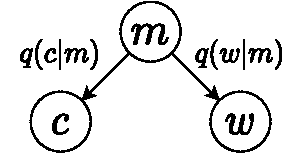
\includegraphics[width=0.4\textwidth]{docs/intro_rate_distortion/graphs/cog_comm_dag.pdf}
    \caption{Illustration of learning problem in a DAG.}
    \label{fig:pipeline_dag}
\end{figure}

The overall objective in the learning part of our project is to plot a trade-off curve like the one shown in Figure~\ref{fig:curve_comm}, but with axes measured by different quantities.
In learning problem, the \textcolor{red}{complexity} is measured by \textcolor{red}{$I(H;C)$}, and the \textcolor{blue}{information loss} is measured by the \textcolor{blue}{negative log-likelihood} of data samples. 


\subsection{Optimisation Objective}
\label{ssec:learn_optim}

In a more formal way, the learning problem is to maximise $P(H|\mathcal{D})$. 
By applying Bayes', we can have the following derivation:
\begin{equation}
    \begin{split}
        p(H|\mathcal{D})
        & \propto p(\mathcal{D}|H)p(H) \\
        & = \prod_{n=1}^{N} p(w_n, c_n|H)p(H)
    \end{split}
    \label{eq:learning_objective_pH_D}
\end{equation}

To achieve this objective, we make another key assumption about $p(w|h)$, i.e. mappings between $H$ and $W$ is also \textcolor{red}{one-to-one}.
Thus, given a pair of $\{w_n, c_n\}\in\mathcal{D}$, we can factorise it as follow:
\begin{equation}
    \begin{aligned}
     & p(w_n, c_n|H) = p(c_n|w_n)p(w_n|h) \\
     & =
        \begin{cases}
            p(c_n|w_n) & \text{if $h=w_n$}\\
            0 & \text{otherwise}
        \end{cases} 
    \end{aligned}
    \label{eq:factorise_data_pair}
\end{equation}

Following our settings in the communication problem, we still assume $p(c_n|w_n)$ is a Gaussian distribution centred at some $\rc(w_n)$.
Then, the probabilistic model illustrated by Figure~\ref{fig:pipeline_dag} could be reduced to a Gaussian mixture model, as shown in the Figure~\ref{fig:learn_gaussian_mix} below.
\begin{figure}[h]
    \centering
    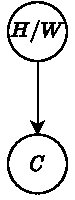
\includegraphics[width=0.1\textwidth]{docs/intro_rate_distortion/graphs/mixture_gaussian.pdf}
    \caption{Model learning problem as a Gaussian mixture model.}
    \label{fig:learn_gaussian_mix}
\end{figure}

To estimate the parameters of this Gaussian mixture model, we can simply use the Expectation–maximisation algorithm\citep{EM} to maximise the likelihood of our data samples.
Then, we can have modes and variances for each $h$, as well as the mixing coefficients. 
More details can be found in the Section 9.2 of \citep{bishop2006pattern}.
Note that the $X$ in Bishop's book should be replaced with $C$, and $Z$ should be replaced with $W$.

\subsection{Trade-off Implied by Maximising a Posterior}
\label{ssec:learn_tradeoff}

Since the logarithm is a monotonic function, the maximum of $P(H|\mathcal{D})$ is also the maximum of $\log P(H|\mathcal{D})$. 
Therefore, to maximise Equation~\ref{eq:learning_objective_pH_D}, it's the same to maximise the following log-likelihood of hypothesis $H$:
\begin{align*}
    % \begin{split}
        & \log p(H|\mathcal{D}) \\
        & \propto \log \prod_{n=1}^{N} p(w_n, c_n|H)p(H) \\
        &  =\sum_{n=1}^{N} \log p(H) p(w_n, c_n|H) \\
        &  =\sum_{n=1}^{N} \log p(H) \log p(w_n, c_n|H) \\
        % &  =\underbrace{N\log p(H)}_{\text{constant, simplicity}} + \underbrace{\sum_{n=1}^{N} \log p(w_n, c_n|H)}_{\text{variable, information loss}} \\
        &  =N\cdot\underbrace{\log p(H)}_{\text{constant}} + \underbrace{\sum_{n=1}^{N} \log p(w_n, c_n|H)}_{\text{variable}} \\
    % \end{split}
    \label{eq:learning_objective_log_pH_D}
\end{align*}

Note that in the above equation, it consists of two terms: 1) $\log p(H)$ which is a constant; 2) $\sum_{n=1}^{N} \log p(w_n, c_n|H)$ is a variable.
Therefore, we can imagine that the number of samples $N$ plays a similar role to the $\beta$ hyper-parameter in the communication problem. 
To be more specific, if $N$ is very small, then the log-likelihood would dominate $\log p(H|\mathcal{D})$, otherwise, $p(H)$ would dominate.

\subsection{Complexity of Hypotheses}
\label{ssec:learn_complexity}

After solving the estimation problem illustrated in Section~\ref{ssec:learn_optim}, for each $h\in\mathcal{H}$, we will have a corresponding mode $\rc(h)$, and variance $\Sigma(h)$. 
At the same time, we will also have a mixing coefficient $\pi_n$ for every $c_n$ in the dataset.
Therefore, we can easily calculate the mutual information between $H$ and $C$ as follow:
\begin{equation}
    I(H;C) = \sum_{h,c} p(c|h)p(h)\log\frac{p(c|h)}{p(c)}
\end{equation}

% Regarding the prior on hypotheses $p(h)$, we can assume an Minimum Description Length prior.
% \textcolor{orange}{@Coleman: can you provide more details about MDL prior?}

We sample $p(H) \sim DP(B, \alpha)$, a Dirichlet-process with given base distribution $B$ and scaling parameter $\alpha$. For Gaussian mixture model $B$ is defined as $\mathcal{N}(\Bar{X},1)$, where $\Bar{X}$ is the mean of the input data (see \ref{ssec:color_dataset}). The scaling parameter $\alpha$ is set to \textit{what?}. Reference for using DP?

For the prior colour-chip distribution we use the least informative prior as defined by \cite{zaslavsky2018efficient}. A single prior distribution is calculated for all languages following the formulation:

\[p(c)=\argmax_{p(c)} H(C)-H_q(C|W)\]

That is, we aim to maximise the uncertainty about our prior colour distribution while minimising the expected uncertainty of $c$ given $w$. Here $H_q(C|W)=-\sum_{c,w} p(c)p(w|c)\log \frac{p(c|w)}{p(c)}$ is the conditional entropy. This formulation is equivalent to mixising the mutual information $I_q(W;C)$ and can be evaluated using the Blahut-Arimoto algorithm. We call this prior the least informative prior because it maximises the expected KL-divergence between prior and posterior:

\begin{align*}
    % \begin{split}
        & I_q(W;C)\\
        &  = \sum_{w,c} p(w)p(c|w)\log \frac{p(c|w)}{p(c)} \\
        &  = \sum_{w} p(w) \sum_c p(c|w)\log \frac{p(c|w)}{p(c)} \\
        &  = \sum_{w} p(w) D[p(c|w)||p(c)] \\
        & = \mathbb{E}_{W}[D[p(c|w)||p(c)]
    % \end{split}
    \label{eq:least_informative_prior}
\end{align*}

simulate actual kid learning
use schedule m
calculate likelihood over all the color chips and average, multiply by N to get number of data points
that is beta for tradeoff

p(H) dirichlet process prior -- favor as few lumps (gaussians) as possible
penalize the gaussian prior on how close the means and std dev
8 terms in english, 8 gaussians, reward gaussians that are basically the same thing
reward gaussian with similar means
reward wider std deviation


ideally variational/dirichlet

generate hypotheses with a schedule, each hypotheses get n data points on the schedule
oversample lower end

information loss not on training data but on WCS data (uniform)

multiply the plot (information loss) by N the number of data points for the hypothesis (dont)

or just plot at N=1 :D

\subsection{Information Loss of Hypotheses}
\label{ssec:learn_info_loss}

In this section, we are going to show why negative log-likelihood could be used as a measure for the information loss in learning problem.
Suppose the distribution of colour chips from dataset $\mathcal{D}$ is $\mathcal{D}(c)$.
Then, we can still used the KL-divergence as a measure for information loss between dataset and the estimated $p(c|H)$.
Considering that $\mathcal{D}(c)$ is still a one-hot distribution, we can factorise the KL-divergence between $\mathcal{D}(c)$ and $p(c|H)$ as follows:
\begin{equation}
    \begin{split}
        D[\mathcal{D}(c)||p(c|H)] & = \sum_{c} \mathcal{D}(c)\log \frac{\mathcal{D}(c)}{p(c|H)} \\
        & = \log \frac{1}{p(c=c_n|H)} \\
        & = -\log p(c=c_n|H)
    \end{split}
    \label{eq:learn_info_loss}
\end{equation}

Therefore, the negative log-likelihood is naturally a measure for the information loss in learning problem.
Fortunately, we would have this quantity once we solve the estimation problem in Section~\ref{ssec:learn_optim}.

\section{Experiment}
\label{sec:experiment}

\subsection{The World Colour Survey Dataset}
\label{ssec:color_dataset}

\begin{table}[h]
\begin{tabular}{lllll}
Language & Speaker & Chip Number & Word &  \\
1        & 1       & 2    & LB   &  \\
1        & 1       & 3    & LE   &  \\
1        & 1       & 4    & WK   &  \\
1        & 1       & 5    & LF   &  \\
1        & 1       & 6    & LE   & 
\end{tabular}
\caption{World Colour Survey sample}
\label{table:raw_data}
\end{table}

The World Colour Survey (WCS) \cite{berlin1991basic} is a global data collection effort that was initiated in the 1970's.
\citet{merrifield1971} theorised about the universality of colour terms in an early paper in 1969 and the WCS was conducted to substantiate these theories.

The colour space was divided into 330 chips of varying colour and intensity (shown in \ref{fig:colour_palette}). 
Multiple native speakers of each language were asked to identify the colour of the chip in their language.
The final dataset includes 110 languages, 2616 speakers, and 2317 unique words.  

An example of the dataset can be seen in Table \ref{table:raw_data}. 
For each language and respective speakers, each colour chip (indicated by a number from 1 to 330) is annotated by a word. 

\begin{table}[h]
\begin{tabular}{llll}
Chip Number & L*    & a*   & b*   \\
141  & 96.00 & -.06 & .06  \\
274  & 91.08 & -.05 & .06  \\
129  & 91.08 & 5.53 & 2.22 \\
230  & 91.08 & 5.51 & 3.28
\end{tabular}
\caption{Predefined mapping from colour chip to the CIELAB perceptual space of colour}
\label{table:lab_values}
\end{table}

The WCS also provides us with a mapping between the chip color space and the CIELAB color space (Table \ref{table:lab_values}).
CIELAB is a colour space designed with the goal of being a perceptually uniform space, where a change in values reflects the same perceived change \cite{CIELAB}.
A visual representation of CIELAB can be seen in Figure \ref{fig:cielab}.
We map colour from chips to the CIELAB space using the mapping provided by the WCS to capture the space of colours in a human perceived space.


\begin{figure}[h]
    \centering
    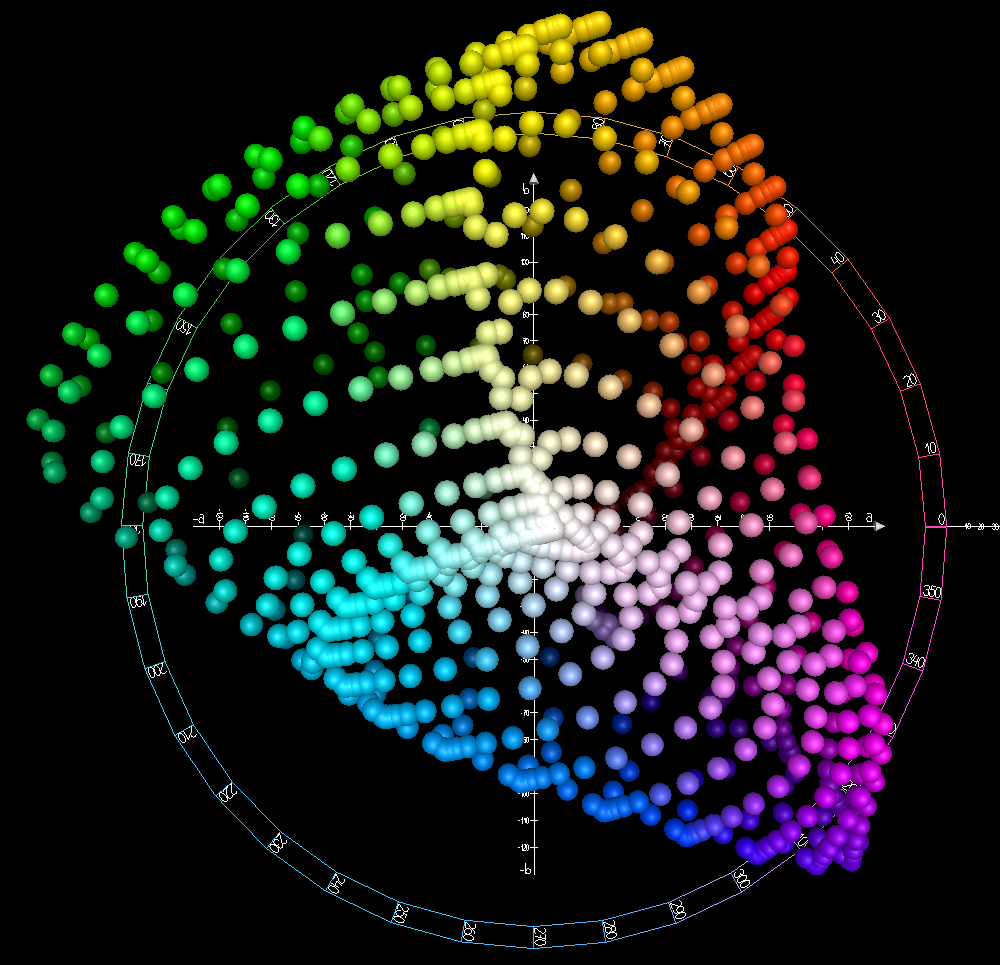
\includegraphics[width=0.3\textwidth]{docs/intro_rate_distortion/graphs/CIELAB_color_space_top_view.png}
    \caption{The CIELAB color space}
    \label{fig:cielab}
\end{figure}


\subsection{Overall Pipeline}
\label{ssec:overall_pipeling}

The procedure of one run for our experiment is illustrated in the following Procedure~\ref{al:exp_procedure}.

\begin{algorithm}[h]
    % \small
    \SetAlgoLined
    \SetAlgorithmName{Procedure}{}
    \KwIn{Input: $\beta$, $N$} \\
    1. [Comm] Set an IB objective with $\beta$; \\
    2. [Comm] Minimise IB objective by optimising $p(w|m)$ and $p(m)$; \\
    3. [Comm] Record complexity $I(M;W)$ and information loss $-I(W;C)$ \\
    3. [Comm] Sample a dataset $\mathcal{D}$ consists of $N$ pairs of $\{w,c\}$ following the distribution $\sum_m p(w|m)p(c|m)p(m)$; \\
    4. [Learn] Fit a Gaussian mixture model on $\mathcal{D}$; \\
    5. [Learn] Record complexity $I(H;C)$ and information loss $-\sum_n\log p(w_n,c_n|H)$.
 \caption{Procedure for one run of experiment. ``Comm'' represent a step in communication problem, and ``Learn'' represents a step in learning problem.}
 \label{al:exp_procedure}
\end{algorithm}

For the values of $\beta$, we can vary it from $1$ to $10$ with step size $0.5$. 
Regard the values of $N$, we can vary it from $20$ to $400$ with step size $20$.
Once we have the complexity and information loss values in both problems for a pair of $(\beta, N)$, we can plot one point in the communication curve like shown in Figure~\ref{fig:curve_comm}, and another point in the learning curve.

\bibliographystyle{acl_natbib}
\bibliography{main}

\end{document}
